\tikzstyle{layer}=[rounded corners=10pt,shading=center]

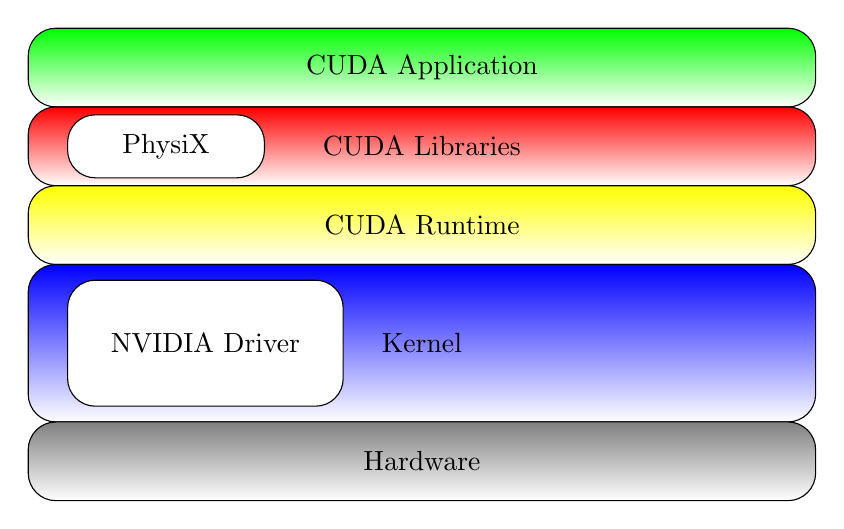
\begin{tikzpicture}
\draw[style=layer,top color=green] (0,0) rectangle (10,1) node[pos=0.5] {CUDA Application};
\draw[style=layer,top color=red] (0,-1) rectangle (10,0) node[pos=0.5] {CUDA
	Libraries};
\draw[style=layer,top color=white] (0.5,-0.9) rectangle (3,-0.1) node[pos=0.5]
{PhysiX};
\draw[style=layer,top color=yellow] (0,-2) rectangle (10,-1) node[pos=0.5] {CUDA
	Runtime};
\draw[style=layer,top color=blue] (0,-4) rectangle (10,-2) node[pos=0.5] {Kernel};
\draw[style=layer,top color=white] (0.5,-3.8) rectangle (4,-2.2) node[pos=0.5]{NVIDIA Driver};
\draw[style=layer,top color=gray] (0.0,-5) rectangle (10,-4) node[pos=0.5]{Hardware};

\end{tikzpicture}
